% --------------------------------------------------------------------------- %
% Poster for the ECCS 2011 Conference about Elementary Dynamic Networks.      %
% --------------------------------------------------------------------------- %
% Created with Brian Amberg's LaTeX Poster Template. Please refer for the     %
% attached README.md file for the details how to compile with `pdflatex`.     %
% --------------------------------------------------------------------------- %
% $LastChangedDate:: 2011-09-11 10:57:12 +0200 (V, 11 szept. 2011)          $ %
% $LastChangedRevision:: 128                                                $ %
% $LastChangedBy:: rlegendi                                                 $ %
% $Id:: poster.tex 128 2011-09-11 08:57:12Z rlegendi                        $ %
% --------------------------------------------------------------------------- %
\documentclass[a0paper,portrait]{baposter}
\usepackage{relsize}		% For \smaller
\usepackage{url}			% For \url
\usepackage{epstopdf}	% Included EPS files automatically converted to PDF to include with pdflatex
\usepackage{lipsum}	% generate non sense text to fill boxes
\usepackage[export]{adjustbox}
\usepackage{enumitem}
\usepackage[none]{hyphenat}

%%% Global Settings %%%%%%%%%%%%%%%%%%%%%%%%%%%%%%%%%%%%%%%%%%%%%%%%%%%%%%%%%%%

\graphicspath{{pix/}}	% Root directory of the pictures
\tracingstats=2			% Enabled LaTeX logging with conditionals

%%% Color Definitions %%%%%%%%%%%%%%%%%%%%%%%%%%%%%%%%%%%%%%%%%%%%%%%%%%%%%%%%%

\definecolor{bordercol}{RGB}{40,40,40}
\definecolor{headercol1}{RGB}{28,144,153}
\definecolor{headercol2}{RGB}{80,80,80}
\definecolor{headerfontcol}{RGB}{0,0,0}
\definecolor{boxcolor}{RGB}{255,255,255} % white

%%%%%%%%%%%%%%%%%%%%%%%%%%%%%%%%%%%%%%%%%%%%%%%%%%%%%%%%%%%%%%%%%%%%%%%%%%%%%%%%
%%% Utility functions %%%%%%%%%%%%%%%%%%%%%%%%%%%%%%%%%%%%%%%%%%%%%%%%%%%%%%%%%%

%%% Save space in lists. Use this after the opening of the list %%%%%%%%%%%%%%%%
\newcommand{\compresslist}{
	\setlength{\itemsep}{1pt}
	\setlength{\parskip}{0pt}
	\setlength{\parsep}{0pt}
}

%%%%%%%%%%%%%%%%%%%%%%%%%%%%%%%%%%%%%%%%%%%%%%%%%%%%%%%%%%%%%%%%%%%%%%%%%%%%%%%
%%% Document Start %%%%%%%%%%%%%%%%%%%%%%%%%%%%%%%%%%%%%%%%%%%%%%%%%%%%%%%%%%%%
%%%%%%%%%%%%%%%%%%%%%%%%%%%%%%%%%%%%%%%%%%%%%%%%%%%%%%%%%%%%%%%%%%%%%%%%%%%%%%%

\begin{document}
\typeout{Poster rendering started}

%%% Setting Background Image %%%%%%%%%%%%%%%%%%%%%%%%%%%%%%%%%%%%%%%%%%%%%%%%%%
%\background{
%	\begin{tikzpicture}[remember picture,overlay]%
%	\draw (current page.north west)+(-2em,2em) node[anchor=north west]
%	{\includegraphics[height=1.1\textheight]{figures/background}};
%	\end{tikzpicture}
%}

%%% General Poster Settings %%%%%%%%%%%%%%%%%%%%%%%%%%%%%%%%%%%%%%%%%%%%%%%%%%%
%%%%%% Eye Catcher, Title, Authors and University Images %%%%%%%%%%%%%%%%%%%%%%
\begin{poster}{
	grid=false,
	columns=5,
	% Option is left on true though the eyecatcher is not used. The reason is
	% that we have a bit nicer looking title and author formatting in the headercol
	% this way
	%eyecatcher=false,
	borderColor=bordercol,
	headerColorOne=headercol1!70,%blue!20,
	headerColorTwo=headercol1!70,%blue!20,
	headerFontColor=headerfontcol,
	% Only simple background color used, no shading, so boxColorTwo isn't necessary
	boxColorOne=boxcolor,
	headershape=roundedright,
	headerfont=\large\sf\bf,
	textborder=faded,%rectangle,
	headerborder=open,
  	boxshade=plain,
	background=plain,%shadetb,
	bgColorOne=white,
	bgColorTwo=blue!10,
	headerheight=6cm
}
%%% Eye Cacther %%%%%%%%%%%%%%%%%%%%%%%%%%%%%%%%%%%%%%%%%%%%%%%%%%%%%%%%%%%%%%%
{

	\includegraphics[width=3cm]{figures/Max-Planck-Gesellschaft.png}

}
%%% Title %%%%%%%%%%%%%%%%%%%%%%%%%%%%%%%%%%%%%%%%%%%%%%%%%%%%%%%%%%%%%%%%%%%%%
{\Large\bf
	MitoBenchStarter: An interactive visual workbench for population genetics on mitochondrial DNA
}
%%% Authors %%%%%%%%%%%%%%%%%%%%%%%%%%%%%%%%%%%%%%%%%%%%%%%%%%%%%%%%%%%%%%%%%%%
{
	\vspace{1em} Judith Neukamm$^{1,3*}$, Alexander Peltzer$^{1,2,3*}$, Wolfgang Haak$^{2}$, Johannes Krause$^{1,2}$ and Kay Nieselt$^{3}$\\
	{\footnotesize \textit{$^1$ Institute for Archaeological Sciences, Archaeo- and Paleogenetics, University of Tuebingen, Germany.\\
	$^2$ Max Planck Institute for the Science of Human History, Jena, Germany.\\
	$^3$ Integrative Transcriptomics, Center for Bioinformatics (ZBIT), University of Tuebingen, Germany.\\
	$*$These authors contributed equally to the work.}\\
	\vspace{1em}
	Contact: judith.neukamm@uni-tuebingen.de
	}
}
%%% Logo %%%%%%%%%%%%%%%%%%%%%%%%%%%%%%%%%%%%%%%%%%%%%%%%%%%%%%%%%%%%%%%%%%%%%%
{
% The logos are compressed a bit into a simple box to make them smaller on the result
% (Wasn't able to find any bigger of them.)
%\setlength\fboxsep{0pt}
%\setlength\fboxrule{0.5pt}

\begin{minipage}{0.15\textwidth}
	\begin{center}
		\includegraphics[width=3cm]{figures/Tuebingen.png}
		%\includegraphics[width=2.5cm]{figures/Pali.png}
	\end{center}
\end{minipage}

	%\fbox{
		%\begin{minipage}{10em}
			%\includegraphics[width=4cm]{figures/it-logo.png}	\\
			%\\
%			\includegraphics[width=3cm]{figures/Max-Planck-Gesellschaft.png}
%

%		\end{minipage}
	%}
}



%---------------------------------------Ha-------------------------------------------------
%	Introduction
%----------------------------------------------------------------------------------------

\headerbox{Motivation \& Goals}{name=introduction, row=0, column=0, span=5}{
		\begin{itemize}[leftmargin=*]
				\item Especially in the research field of ancient human DNA, mitochondrial DNA (mtDNA) is often the only proxy available to study extinct populations and their relationship with modern populations
				\item Tools for the analysis typically rely on different file formats $\rightarrow$ requires manual interaction with the data for downstream analysis
				\item mitoBench: workbench to ease file conversions, interactively analyze human mitochondrial genomes and visualize results
				\item mitoDB: database for mitochondrial reference data to provide a central reference database that can be easily accessed via the workbench
		\end{itemize}

}


%----------------------------------------------------------------------------------------
%  Workflow
%----------------------------------------------------------------------------------------


\headerbox{Workflow}{name=workflow, column=0, span=2, below=introduction}{
	\centering
	\includegraphics[width=0.8\textwidth]{figures/workflow_yed.jpg}

}

%----------------------------------------------------------------------------------------
%	MitoDB
%----------------------------------------------------------------------------------------


\headerbox{mitoDB}{name=mitodb, row=1, column=2, span=3, below=introduction, bottomaligned=workflow}{

	\begin{minipage}{0.8\textwidth}
		\begin{itemize}
			\item Web-Frontend with Vaadin Java Framework
			\item Backend with PostgreSQL, providing sequence information and meta-data
			\item Curated data upload with meta-data
			\item Retrieval possible through WebUI and mitoBench
		\end{itemize}
	\end{minipage}
	\begin{minipage}{0.15\textwidth}
		\begin{center}
			\includegraphics[width=2cm]{figures/postgresql.png}
			\vspace{2em}
			\includegraphics[width=0.1\paperwidth]{figures/vaadin.png}
		\end{center}
	\end{minipage}

}



%----------------------------------------------------------------------------------------
%	Mitobench
%----------------------------------------------------------------------------------------


\headerbox{mitoBench}{name=mitobench, column=0, span=3,below=workflow}{
	\begin{minipage}[t]{0.5\textwidth}
		\textbf{File conversions}\\
		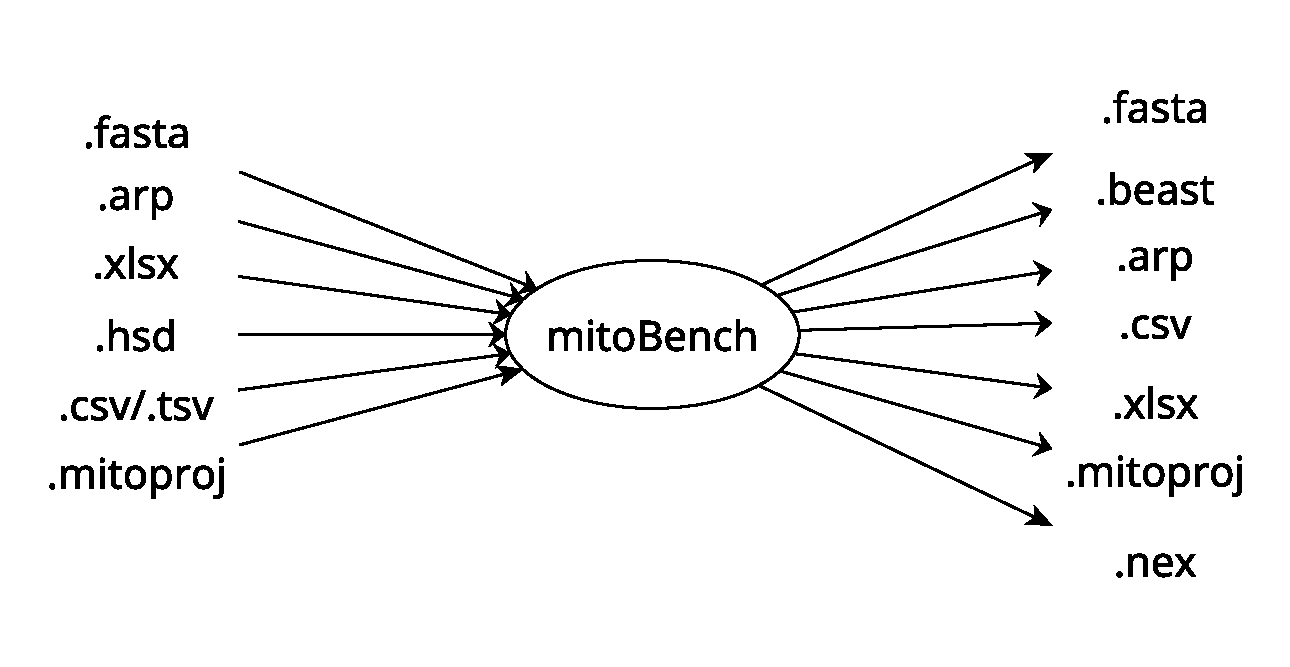
\includegraphics[width=0.8\textwidth, left]{figures/import_export.jpg}
		$\Rightarrow$ connect the workbench with existing analysis methods such as BEAST, Arlequin, PhyloTree and others
	\end{minipage}
	\hspace{0.5em}
	\begin{minipage}[t]{0.5\textwidth}
		\textbf{Data representation as Table}\\
		\\
		\includegraphics[width=0.85\textwidth, left]{figures/load_generic.png}
	\end{minipage}

	\vspace{2em}

	\begin{minipage}[t]{0.5\textwidth}
		\textbf{Data grouping}
		\begin{itemize}[leftmargin=*]
			\item group data based on shared feature \\
			(e.g. time period, location)
			\item user defined grouping
		\end{itemize}
		$\Rightarrow$ allows analysis of Haplogroup distribution between different groups
	\end{minipage}
	\hspace{0.5em}
	\begin{minipage}[t]{0.5\textwidth}
		\textbf{Data filtering / Statistics}
		\begin{itemize}[leftmargin=*]
			\item Haplogroup filtering / frequencies
			\item Mutation filtering / frequencies
		\end{itemize}
		Haplogroups based on \includegraphics[width=2cm]{figures/phylotree.png}
	\end{minipage}

	\vspace{2em}

	\begin{minipage}[t]{0.5\textwidth}
		\textbf{Data visualizations}\\
		\\
		\includegraphics[width=\textwidth, left]{figures/stackedBarchart.png}
	\end{minipage}
	\hspace{0.5em}
	\begin{minipage}[t]{0.5\textwidth}
		\textbf{}\\
		\\
		\includegraphics[width=0.9\textwidth, left]{figures/profile.png}
	\end{minipage}

	\vspace{2em}

	\begin{minipage}[t]{0.5\textwidth}
		\textbf{}\\
		\includegraphics[width=0.85\textwidth, center]{figures/sunburst3.png}
	\end{minipage}
	\hspace{0.5em}
	\begin{minipage}[t]{0.5\textwidth}
		\textbf{}\\
		\\
		\includegraphics[width=0.9\textwidth, left]{figures/group_sizes.png}
	\end{minipage}

}


%----------------------------------------------------------------------------------------
%	Outlook
%----------------------------------------------------------------------------------------

\headerbox{Outlook}{name=outlook,row=0, column=3, span=2,  below=mitodb}{
	\textbf{mitoBench}
	\begin{itemize}
		\item Provide methods for downstream analysis \\
		(e.g. F$_{ST}$ calculations, Founder Analysis)
		\item Offer more visualizations (e.g. geographical maps)\\
		\\
		\hspace{1em}\includegraphics[width=0.5\textwidth]{figures/map.png}
	\end{itemize}
	\textbf{mitoDB \& web interface}
	\begin{itemize}
		\item Export/import functionality
		\item web-based dashboard to explore database\\
		\\
		\includegraphics[width=0.7\textwidth]{figures/mitodb_dashboard.png}
	\end{itemize}

}


%----------------------------------------------------------------------------------------
%	References
%----------------------------------------------------------------------------------------

\headerbox{References}{name=references, column=3, span=2, above=bottom, below=outlook}{
	\scriptsize
	\begin{enumerate}[topsep=0pt,itemsep=-1ex,partopsep=1ex,parsep=1ex]
			\item Drummond, A. J., Suchard, M. A., Xie, D., \& Rambaut, A. (2012). Bayesian phylogenetics with BEAUti and the BEAST 1.7. \textit{Molecular biology and evolution}, 29(8), 1969-1973.
			\item Excoffier, L., \& Lischer, H. E. (2010). Arlequin suite ver 3.5: a new series of programs to perform population genetics analyses under Linux and Windows. \textit{Molecular ecology resources}, 10(3), 564-567.
			\item Van Oven, M., \& Kayser, M. (2009). Updated comprehensive phylogenetic tree of global human mitochondrial DNA variation. \textit{Human mutation}, 30(2), E386-E394.
			\item Weissensteiner, H., Pacher, D., Kloss-Brandst\"atter, A., Forer, L., Specht, G., Bandelt, H. J., ... \& Sch\"onherr, S. (2016). HaploGrep 2: mitochondrial haplogroup classification in the era of high-throughput sequencing. \textit{Nucleic acids research}, gkw233.
	\end{enumerate}
}


\end{poster}
\end{document}
